\documentclass[a4paper,12pt]{article}

% Need \centerdot
\usepackage{amssymb}

% Set margins
\usepackage{geometry}
\geometry{
  top=1.0cm,            % <-- you want to adjust this
  inner=1.5cm,
  outer=1.5cm,
  bottom=1.0cm,
  headheight=3ex,       % <-- and this
  headsep=2ex,          % <-- and this
}

% No page numbers
\pagestyle{empty}

% Set paragraph indent to 2.2mm, even first
\usepackage{indentfirst}
\setlength{\parindent}{2.2mm}

% Image support
\usepackage{graphicx}

% Need \XeLaTex logo
\usepackage{xltxtra}

% Set font to Garamond
\usepackage{fontspec}
\setmainfont[Numbers=OldStyle,
	     Scale=1.05,
	     ItalicFont={Adobe Garamond Pro Italic},
             BoldFont={Adobe Garamond Pro Semibold}
            ]{Adobe Garamond Pro}

% Set section to MidnightBlue with horizontal rule
\usepackage[dvipsnames,usenames]{color}
\usepackage[explicit]{titlesec}
\titleformat{\section}[display]{\Large\color{MidnightBlue}}{\thetitle}{1em}{#1}[{\titlerule}]

% Text layout commands
\newcommand{\topSection}[2]
{
	\begin{minipage}[b]{0.68\textwidth} #1 \end{minipage}
	\begin{minipage}[t]{0.28\textwidth} #2 \end{minipage}
	\vspace{0.4\baselineskip}
}

\newcommand{\standardEntry}[2]
{
	\vspace{0.4\baselineskip}
	\begin{minipage}[t]{0.25\textwidth} {\small \textsc{#1}} \end{minipage}
	\begin{minipage}[t]{0.725\textwidth} #2 \end{minipage}
	\par
}

\newcommand{\stretchedEntry}[2]
{
	\vspace{0.4\baselineskip}
	#1 \hfill #2
	\vspace{\baselineskip}
	\par
}

\newcommand{\indentedEntry}[2]
{
	\standardEntry{\hspace{0.125\textwidth} #1}{#2}
}


\begin{document}

\topSection
{
	{\Huge Jorge Azevedo}

	\vspace{1.5mm}
	\resizebox{4.9cm}{!}{\textit{Software Engineer}}
	\vspace*{10mm}

	\textbf{Job applied for}: Junior Software Developer

	\textbf{Availability}: March 2014 onwards
} {
	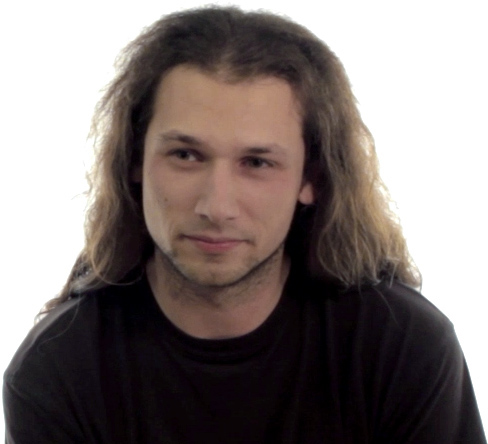
\includegraphics[width=0.985\textwidth]{img/photo}
}

\emph{In a nutshell} $\cdot$ Software engineer with 2 years experience looking
to integrate into a high-performing team developing quality software.
Specialties include test-driven development and GNU/Linux.

\section*{Personal Information}

\standardEntry{Full name}{Jorge Manuel Coelho Amado de Azevedo}
\standardEntry{Nationality}{Portuguese} 
\standardEntry{Date of Birth}{15th October 1987}
\standardEntry{Contacts}
{
% @{} removes the table's left side indentation
\begin{tabular}[t]{@{}l l}
	$\cdot$  Address & Luxemburger Straße 30, 13353 Berlin, Germany \\
	$\cdot$  Telephone & (+351) 936270876 \\
	$\cdot$  E-mail & \href{mailto:jorge.amado.azevedo@gmail.com}{jorge.amado.azevedo@gmail.com} \\
	$\cdot$  Skype & jorge.amado.azevedo\\
	$\cdot$  LinkedIn & \href{http://pt.linkedin.com/in/jaazevedo}{pt.linkedin.com/in/jaazevedo}\\
\end{tabular}
}

\section*{Experience}

\stretchedEntry{UnlockYourBrain}{Berlin, Germany}
\indentedEntry{Aug 2013 - Jan 2014}{\textbf{Software Engineer}}
\indentedEntry{Description}
{
Freelance engineer at UnlockYourBrain, an e-learning startup focused on the development
of an Android app with over 300K downloads. Key projects:

$\cdot$  Continuous integration of the Android app using TeamCity and Gradle.

$\cdot$  Implementation of Scrum. As Scrum Master I oversaw the
adoption of the framework, scheduled and hosted  the various events, etc.

}

\vspace{\baselineskip}
\stretchedEntry{UNISOL}{University of Aveiro, Portugal}
\indentedEntry{Mar 2012 - Jul 2013}{\textbf{Researcher}}
\indentedEntry{Description}
{
Research grant for UNISOL, a European consortium purposed with the construction
of a domestic solar heating system. Key projects:

$\cdot$  Embedded control system using a PIC32 and tens of sensors and
actuators.

$\cdot$  Deployment and administration of an Ubuntu server running an
OpenStack cloud computing environment and a MATLAB computation cluster.
}

\vspace{\baselineskip}
\stretchedEntry{Xenomai Lab}{University of Aveiro, Portugal}
\indentedEntry{Jan 2011 - Jul 2013}{\textbf{Software Developer}}
\indentedEntry{Description}
{
A Linux real-time platform I developed for my thesis and continued to work on as a
researcher. Technical coordinator for two student master's thesis.

$\cdot$  Qt/C++ GUI for designing control systems using Xenomai C real-time tasks.

$\cdot$ Sept 2012 - Dez 2013 \emph{Control teaching platform based on Xenomai Lab}.

$\cdot$ Jan 2012 - Dez 2012 \href{http://ria.ua.pt/handle/10773/10933}{\emph{Adaptive Controller based on Xenomai Lab}}.
}

\section*{Publications}

\standardEntry{Sept 2012}{\href{http://inforum.org.pt/INForum2012/docs/20120576.pdf/at_download/file}{Xenomai Lab - A Platform for Digital Real-Time
Control} (\href{http://inforum.org.pt/INForum2012/docs/20120576.pdf/at_download/file}{\underline{link}})} \standardEntry{In}{J. Amado-Azevedo, P. Pedreiras and A. Mota.
\emph{Xenomai Lab - A Platform for Digital Real-time Control}. In INForum
Proceedings, 2012.}

\section*{Education}

\standardEntry{Sept 2005 – Jan 2012}{\textbf{M.Sc. Electronics and Telecommunications
Engineering}}
\standardEntry{Institution}
{
\textbf{University of Aveiro, Portugal}
}
\standardEntry{Thesis}{\href{http://ria.ua.pt/bitstream/10773/8582/1/248569.pdf}{Xenomai Lab - A Platform For Digital Real-Time Control} (\href{http://ria.ua.pt/bitstream/10773/8582/1/248569.pdf}{\underline{link}})}
\standardEntry{Description}
{
5 year program including Bachelor's and Master's. Thesis graded 19/20.
}

\vspace{\baselineskip}

\standardEntry{Sept 2008 – Jul 2009}{\textbf{Erasmus Exchange Program}}
\standardEntry{Institution}
{
\textbf{TU\textbackslash e Technische Universiteit Eindhoven, Netherlands}
}
\standardEntry{Description}
{
One year spent abroad under the Erasmus Exchange Program.
}

\section*{Languages}

\standardEntry{Portuguese}{Native speaker.}
\standardEntry{English}
{
Fluent speaker. Six years of education in the British Council achieving level
B in the Certificate of Advanced English (2004).
}
\standardEntry{Spanish}{Basic understanding in both written and spoken form.}


\section*{Skills}

\standardEntry{Software}
{
 $\cdot$ A thorough understanding of the C programming language and Real-Time OS
semantics, based on Linux variants such as Xenomai and RTAI.

 $\cdot$ Comfortable with Node.JS, C++/Qt, Android and iOS development.

 $\cdot$ Practioner of TDD, Continuous Integration (Jenkins, TeamCity), cloud
computing (OpenStack).
}
\standardEntry{Hardware}
{
 $\cdot$ A working knowledge of PIC microcontrollers, basic analog filter design and PCB
prototyping using EAGLE.
}
\standardEntry{Social}
{
 $\cdot$ Experience integrating into foreign and multicultural environments.

 $\cdot$ Open minded and empathetic presence in a team.
}
\standardEntry{Organizational}
{

 $\cdot$ Experience in the Scrum framework as both a Developer and Scrum
Master.

 $\cdot$ Synthesis and automation of workflows inside a team, e.g.
translation deployment, git branching models, etc.
}

\standardEntry{Others}{ $\cdot$ Driving License Category B-1}

\vfill

\begin{center}
{
    \scriptsize  Last updated: \today ~$\cdot$ Typeset in \XeLaTeX\\
    http://github.com/jorgeazevedo/jorge-azevedo-cv
}

\end{center}
\end{document}
